% CELLAIR Elevator Pitch — University of Salzburg
% Compile with: pdflatex main.tex (twice for references)
\documentclass[aspectratio=169,11pt]{beamer}

% ============================================================
% Theme: Clean, minimal
% ============================================================
\usetheme{default}
\usecolortheme{default}

% Colors — University of Salzburg corporate design
\definecolor{unisalz}{RGB}{17, 87, 64}         % Grün PANTONE 343 C
\definecolor{unisalzgray}{RGB}{156, 156, 156}   % Grau PANTONE Cool Grey 9
\definecolor{unisalzlight}{RGB}{214, 232, 226}  % light green tint (accents)
\definecolor{alertred}{RGB}{180, 40, 40}        % alert/warning

\setbeamercolor{structure}{fg=unisalz}
\setbeamercolor{frametitle}{fg=unisalz, bg=white}
\setbeamercolor{title}{fg=unisalz}
\setbeamercolor{subtitle}{fg=unisalzgray}
\setbeamercolor{author}{fg=unisalzgray}
\setbeamercolor{date}{fg=unisalzgray}
\setbeamercolor{institute}{fg=unisalzgray}
\setbeamercolor{normal text}{fg=black, bg=white}
\setbeamercolor{block title}{fg=white, bg=unisalz}
\setbeamercolor{block body}{bg=unisalzlight}
\setbeamercolor{alerted text}{fg=alertred}
\setbeamercolor{headlinecolor}{fg=unisalzgray, bg=white}
\setbeamercolor{footlinecolor}{fg=unisalzgray, bg=white}

% Remove navigation symbols
\setbeamertemplate{navigation symbols}{}

% ============================================================
% Header: logo + "University of Salzburg" left | "AG Lepperdinger" + date right
% ============================================================
\setbeamertemplate{headline}{%
  \begin{beamercolorbox}[wd=\paperwidth, ht=0.55cm, dp=0.2cm]{headlinecolor}%
    \hspace{0.6em}%
    \raisebox{0.05cm}{
\includegraphics[height=0.38cm]{img/Siegel-300x300-corpgrey.png}}%
    \hspace{0.25em}%
    \raisebox{0.12cm}{{\small\color{unisalzgray} universit\"{a}t}%
    {\small\color{unisalz}\bfseries\rmfamily salzburg}}%
    \hfill%
    {\small\color{unisalzgray}AG Lepperdinger}%
    \hspace{2.0em}%
  \end{beamercolorbox}%
  \begin{beamercolorbox}[wd=\paperwidth, ht=0.4pt]{structure}%
  \end{beamercolorbox}%
}

% ============================================================
% Footer: page x/y left | frame subtitle center-right
% ============================================================
\setbeamertemplate{footline}{%
  \begin{beamercolorbox}[wd=\paperwidth, ht=0.4pt]{structure}%
  \end{beamercolorbox}%
  \begin{beamercolorbox}[wd=\paperwidth, ht=0.45cm, dp=0.2cm]{footlinecolor}%
    \hspace{0.6em}%
    {\footnotesize\color{unisalzgray}%
      \insertframenumber\,/\,\inserttotalframenumber}%
    \hfill%
    {\footnotesize\color{unisalzgray}\usebeamertemplate{frame subtitle}}%
    \hspace{0.6em}%
  \end{beamercolorbox}%
}

% ============================================================
% Packages
% ============================================================
\usepackage[utf8]{inputenc}
\usepackage[T1]{fontenc}
\usepackage{lmodern}
\usepackage{graphicx}
\usepackage{booktabs}
\usepackage{multirow}
\usepackage{amsmath}
\usepackage[version=4]{mhchem}
\usepackage{siunitx}
\usepackage{tikz}
\usepackage{hyperref}
\usepackage[useregional=false,datesep=-]{datetime2}

\sisetup{per-mode=symbol}

% ============================================================
% University wordmark — corporate design
% "universität" in grey, "salzburg" in green bold
% ============================================================
\newcommand{\uniwordmark}{%
  {\color{unisalzgray}\rmfamily universit\"{a}t}%
  {\color{unisalz}\bfseries\rmfamily salzburg}%
}

% ============================================================
% Title page data
% ============================================================
\title{CELLAIR Mesoscope}
\subtitle{CELL Analysis with Intelligent Recognition}
\author[Florian Feigl]{Florian Feigl}
\institute{University of Salzburg}
\date{\DTMtoday}

% ============================================================
% Document
% ============================================================
\begin{document}

% --------------------------------------------------
% Title
% --------------------------------------------------
\begin{frame}[plain]
  \centering
  \vspace{2em}
  {\huge\color{unisalz}\bfseries CELLAIR Mesoscope\par}
  \vspace{0.8em}
  {\large\color{unisalzgray} CELL Analysis with Intelligent Recognition\par}
  \vspace{2em}
  {\large Florian Feigl\par}
  \vspace{1.5em}
  \begin{tabular}{m{1.2cm}m{3cm}}
    
\includegraphics[height=1.2cm]{img/Siegel-300x300-corpgrey.png} &
    {\Large\color{unisalzgray} universit\"{a}t}\\[-0.2em]
    {\Large\color{unisalz}\bfseries salzburg}
  \end{tabular}\par
  \vspace{1.5em}
  {\small\color{unisalzgray}\DTMtoday\par}
\end{frame}

% --------------------------------------------------
% Slide 1: What We Observe
% --------------------------------------------------
\begin{frame}{What We Observe}

  \textbf{Calcium production through cell--cell interaction}

  \begin{itemize}
    \item \textbf{hFOB~1.19} (human fetal osteoblasts) and \textbf{hMEC~1} (human microvascular endothelial cells)
    \item Osteoblasts produce \textbf{hydroxyapatite} (\ce{Ca10(PO4)6(OH)2}) --- the mineral component of bone
    \item Key question: How do endothelial cells influence and respond to osteoblast mineralization?
  \end{itemize}

  \vfill
  \small
  Relevant for bone tissue engineering, implant osseointegration, and regenerative medicine.

\end{frame}

% --------------------------------------------------
% Slide 2: Technical Approach
% --------------------------------------------------
\begin{frame}{Technical Approach --- Simulating the Natural Environment}

  \begin{center}
  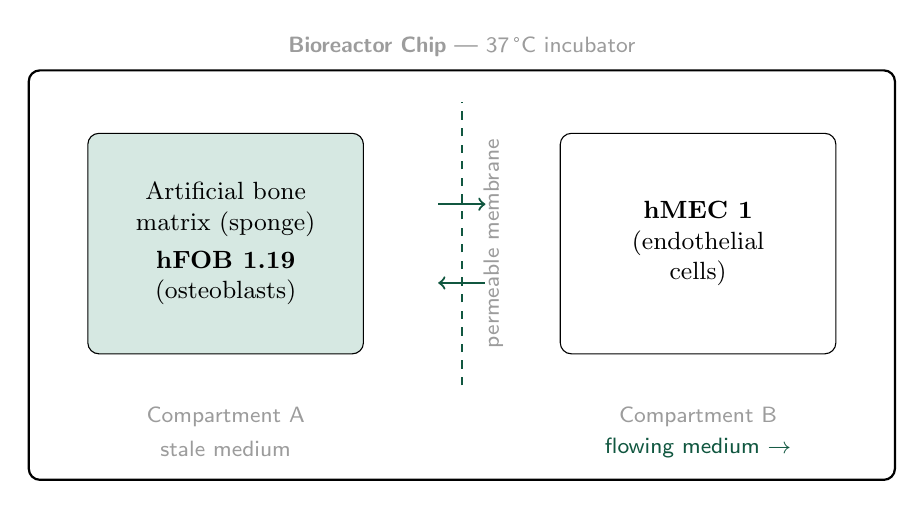
\begin{tikzpicture}[
    comp/.style={draw, rounded corners, minimum width=3.5cm, minimum height=2.8cm, align=center, font=\small},
    membrane/.style={draw, dashed, thick, color=unisalz},
    label/.style={font=\footnotesize\sffamily, color=unisalzgray}
  ]
    % Compartments
    \node[comp, fill=unisalzlight] (compA) at (-3, 0) {Artificial bone\\matrix (sponge)\\[0.3em]\textbf{hFOB 1.19}\\(osteoblasts)};
    \node[comp, fill=white] (compB) at (3, 0) {\textbf{hMEC 1}\\(endothelial\\cells)};

    % Membrane
    \draw[membrane] (0, -1.8) -- (0, 1.8);
    \node[label, rotate=90] at (0.4, 0) {permeable membrane};

    % Arrows through membrane
    \draw[->, thick, color=unisalz] (-0.3, 0.5) -- (0.3, 0.5);
    \draw[<-, thick, color=unisalz] (-0.3, -0.5) -- (0.3, -0.5);

    % Labels
    \node[label] at (-3, -2.2) {Compartment A};
    \node[label] at (3, -2.2) {Compartment B};
    \node[label] at (-3, -2.6) {stale medium};
    \node[label, color=unisalz] at (3, -2.6) {flowing medium $\rightarrow$};

    % Outer box
    \draw[thick, rounded corners] (-5.5, -3.0) rectangle (5.5, 2.2);
    \node[label] at (0, 2.5) {\textbf{Bioreactor Chip} --- 37\,°C incubator};
  \end{tikzpicture}
  \end{center}

  \vfill
  \small
  Flow rate: TBD (depends on chip geometry and shear stress tolerance)

\end{frame}

% --------------------------------------------------
% Slide 3: Current Status
% --------------------------------------------------
\begin{frame}{Current Status --- What We Have}

  \textbf{General experiment structure established.}\\
  Bringing specimen and observation unit in place for early stage evaluation.

  \vspace{0.5em}

  \begin{tabular}{@{}lll@{}}
    \toprule
    \textbf{Component} & \textbf{Status} \\
    \midrule
    Bioreactor chip design        & Established \\
    Cell lines (hFOB~1.19, hMEC~1) & Available \\
    Computing (RPi~5 + Hailo-8 NPU) & Operational \\
    HQ Camera (IMX477, C-mount)   & Acquired \\
    OpenFlexure server (v3)       & Running \\
    \bottomrule
  \end{tabular}

  \vspace{0.8em}
  \small
  Currently verifying imaging quality on conventional microscope before transitioning to OpenFlexure platform.

\end{frame}

% --------------------------------------------------
% Slide 4: OpenFlexure Hardware
% --------------------------------------------------
\begin{frame}{OpenFlexure Microscope --- Hardware Platform}

  \begin{columns}[T]
    \begin{column}{0.45\textwidth}
      \textbf{Open-source, 3D-printed}\\
      \textbf{motorised microscope}\\[0.3em]
      \small Cambridge, CERN-OHL license

      \vspace{0.8em}

      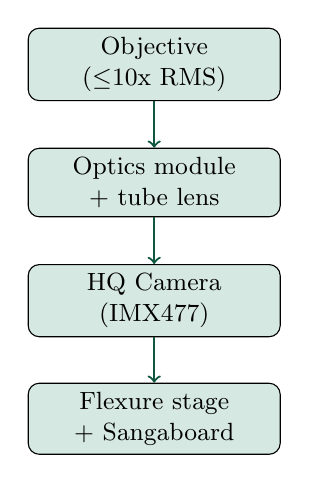
\begin{tikzpicture}[
        box/.style={draw, rounded corners, minimum width=3.2cm, align=center, font=\small, fill=unisalzlight},
        arrow/.style={->, thick, color=unisalz}
      ]
        \node[box] (obj) at (0, 4.5) {Objective\\($\leq$10x RMS)};
        \node[box] (optics) at (0, 3.0) {Optics module\\+ tube lens};
        \node[box] (cam) at (0, 1.5) {HQ Camera\\(IMX477)};
        \node[box] (stage) at (0, 0) {Flexure stage\\+ Sangaboard};
        \draw[arrow] (obj) -- (optics);
        \draw[arrow] (optics) -- (cam);
        \draw[arrow] (cam) -- (stage);
      \end{tikzpicture}
    \end{column}

    \begin{column}{0.52\textwidth}
      \textbf{Pending hardware:}

      \vspace{0.3em}

      \begin{tabular}{@{}ll@{}}
        \toprule
        \textbf{Part} & \textbf{Status} \\
        \midrule
        Sangaboard v5            & On order \\
        Stepper motors (3x)      & On order \\
        Bag of Bits (hardware)   & On order \\
        Illumination kit         & On order \\
        Tube lens (125--150\,mm) & On order \\
        Custom optics STL        & In dev. \\
        \bottomrule
      \end{tabular}

      \vspace{0.8em}
      \small
      All parts ordered via Taulab / distributor.\\
      Custom optics module compiled from OpenSCAD source.
    \end{column}
  \end{columns}

\end{frame}

% --------------------------------------------------
% Slide 5: The 25% Problem
% --------------------------------------------------
\begin{frame}{Why Custom Optics --- The Sensor Utilization Problem}

  Standard OpenFlexure tube lens (50\,mm) was designed for Pi Camera~v2 (4.6\,mm diagonal).\\
  Our HQ Camera IMX477 has a \textbf{9.79\,mm diagonal --- 2.1$\times$ larger}.

  \vspace{0.5em}

  \begin{columns}[T]
    \begin{column}{0.55\textwidth}
      \begin{tabular}{@{}lrrr@{}}
        \toprule
        \textbf{Tube lens} & \textbf{M} & \textbf{EFN} & \textbf{Sensor used} \\
        \midrule
        50\,mm (std.)   & 0.261 & 37.5\,mm & \alert{$\sim$25\%} \\
        125\,mm         & 0.469 & 20.9\,mm & $\sim$85\% \\
        150\,mm         & 0.515 & 19.0\,mm & $\sim$95\% \\
        \bottomrule
      \end{tabular}
    \end{column}

    \begin{column}{0.42\textwidth}
      \small
      \textbf{Calculation:}
      \begin{align*}
        M &= \frac{f_t}{f_t + |p|} \\[0.3em]
        \text{Area ratio} &= \left(\frac{4.6}{9.79}\right)^2 \approx 22\%
      \end{align*}

      \vspace{0.3em}
      $p = -141.5$\,mm (back focal length)\\
      EFN = effective field number
    \end{column}
  \end{columns}

  \vfill
  \textbf{Solution:} Replace 50\,mm tube lens with \textbf{125--150\,mm achromatic doublet} (same 12.7\,mm diameter). Requires custom optics module STL.

\end{frame}

% --------------------------------------------------
% Slide 6: Prospect 1 --- Data Quality
% --------------------------------------------------
\begin{frame}{Prospect \#1 --- Enhancing Data Quality}

  \textbf{Equipping experimental base setup with high-quality compounds}

  \vspace{0.5em}

  \begin{tabular}{@{}lll@{}}
    \toprule
    \textbf{Upgrade} & \textbf{Purpose} & \textbf{Impact} \\
    \midrule
    Custom optics module   & Match tube lens to IMX477  & Full sensor utilization \\
    $\leq$10x RMS objective & Cell-level observation     & $\sim$1.3\,\si{\micro\meter} at 10x \\
    Flat-field correction  & Even illumination          & Consistent intensity \\
    Motorised stage        & Sub-\si{\micro\meter} positioning & Automated time-lapse \\
    \bottomrule
  \end{tabular}

  \vfill
  \textbf{Result:} Higher quality raw data $\rightarrow$ better annotation $\rightarrow$ better model performance

\end{frame}

% --------------------------------------------------
% Slide 7: Prospect 2 --- Automated Recognition
% --------------------------------------------------
\begin{frame}{Prospect \#2 --- Automated Event Recognition}

  \textbf{Event-sensitive cell--cell interaction recognition via NPU inference}

  \vspace{0.3em}

  \begin{center}
  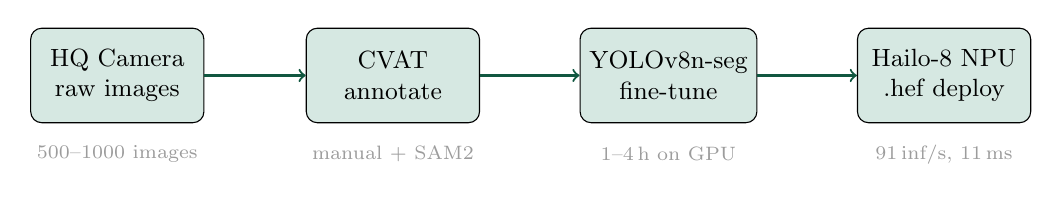
\begin{tikzpicture}[
    box/.style={draw, rounded corners, minimum width=2.2cm, minimum height=1.2cm, align=center, font=\small, fill=unisalzlight},
    arrow/.style={->, thick, color=unisalz}
  ]
    \node[box] (cam) at (0, 0) {HQ Camera\\raw images};
    \node[box] (cvat) at (3.5, 0) {CVAT\\annotate};
    \node[box] (yolo) at (7, 0) {YOLOv8n-seg\\fine-tune};
    \node[box] (hailo) at (10.5, 0) {Hailo-8 NPU\\.hef deploy};
    \draw[arrow] (cam) -- (cvat);
    \draw[arrow] (cvat) -- (yolo);
    \draw[arrow] (yolo) -- (hailo);

    \node[font=\scriptsize, color=unisalzgray] at (0, -1.0) {500--1000 images};
    \node[font=\scriptsize, color=unisalzgray] at (3.5, -1.0) {manual + SAM2};
    \node[font=\scriptsize, color=unisalzgray] at (7, -1.0) {1--4\,h on GPU};
    \node[font=\scriptsize, color=unisalzgray] at (10.5, -1.0) {91\,inf/s, 11\,ms};
  \end{tikzpicture}
  \end{center}

  \vspace{0.3em}

  \begin{columns}[T]
    \begin{column}{0.48\textwidth}
      \small
      \textbf{Target classes:}
      \begin{itemize}
        \item Osteoblasts
        \item Endothelial cells
        \item Mineralization zones
        \item Membrane boundary
      \end{itemize}
    \end{column}
    \begin{column}{0.48\textwidth}
      \small
      \textbf{Annotation effort:}
      \begin{tabular}{@{}lr@{}}
        \toprule
        Method & Time/image \\
        \midrule
        Manual       & 5--10\,min \\
        SAM2-assisted & 1--3\,min \\
        \bottomrule
      \end{tabular}

      \vspace{0.3em}
      500 images $\approx$ 8--42\,h\\
      1000 images $\approx$ 17--83\,h
    \end{column}
  \end{columns}

\end{frame}

% --------------------------------------------------
% Slide 8: Data Storage
% --------------------------------------------------
\begin{frame}{Data Storage --- Raw Image Estimates}

  \textbf{IMX477 sensor:} 4056\,$\times$\,3040 pixels, 12.3\,MP

  \vspace{0.5em}

  \begin{columns}[T]
    \begin{column}{0.48\textwidth}
      \begin{tabular}{@{}lrrr@{}}
        \toprule
        \textbf{Format} & \textbf{/image} & \textbf{500} & \textbf{1000} \\
        \midrule
        12-bit RAW  & 18.5\,MB & 9.2\,GB  & 18.5\,GB \\
        16-bit TIFF & 24.7\,MB & 12.3\,GB & 24.7\,GB \\
        JPEG (HQ)   & 8\,MB    & 4.0\,GB  & 8.0\,GB \\
        \bottomrule
      \end{tabular}
    \end{column}
    \begin{column}{0.48\textwidth}
      \textbf{Time-lapse (48\,h):}

      \begin{tabular}{@{}lrr@{}}
        \toprule
        \textbf{Interval} & \textbf{Frames} & \textbf{RAW} \\
        \midrule
        1\,min  & 2880 & 53\,GB \\
        5\,min  & 576  & 11\,GB \\
        10\,min & 288  & 5\,GB \\
        \bottomrule
      \end{tabular}
    \end{column}
  \end{columns}

  \vfill

  \begin{block}{Recommendation}
    Attach \textbf{USB~3.0 SSD (256\,GB+)} to RPi~5 for raw data collection.
    Back up to NAS after each session.
    SD card (32\,GB) is \emph{not} sufficient for RAW time-lapse series.
  \end{block}

\end{frame}

% --------------------------------------------------
% Slide 9: Goal 1
% --------------------------------------------------
\begin{frame}{Goal \#1 --- Biological Insight}

  \textbf{Gaining deeper insight into cell--cell interaction dynamics\\ during hydroxyapatite production}

  \vspace{0.5em}

  \begin{itemize}
    \item How does proximity to active osteoblasts affect endothelial cell morphology and migration?
    \item Does the rate of calcium deposition change in the presence of endothelial signaling?
    \item Can we identify temporal patterns --- do interactions follow predictable phases?
    \item What morphological markers precede mineralization events?
  \end{itemize}

  \vfill
  \textbf{Measurement approach:}
  \begin{itemize}
    \item Automated time-lapse imaging (hours to days)
    \item AI-assisted segmentation of cell populations and mineralization zones
    \item Quantitative tracking: cell count, area, migration velocity, mineralization density
  \end{itemize}

\end{frame}

% --------------------------------------------------
% Slide 10: Goal 2
% --------------------------------------------------
\begin{frame}{Goal \#2 --- Autonomous Reproducibility}

  \textbf{Building a stable, reproducible experimental platform}

  \vspace{0.5em}

  \begin{tabular}{@{}ll@{}}
    \toprule
    \textbf{Requirement} & \textbf{Solution} \\
    \midrule
    Hardware reproducibility  & Open-source 3D-printed microscope (CERN-OHL) \\
    Software reproducibility  & Ansible-automated deployment ($<$10\,min) \\
    Protocol reproducibility  & Scripted sessions via OpenFlexure REST API \\
    Analysis reproducibility  & Compiled .hef model --- deterministic inference \\
    \bottomrule
  \end{tabular}

  \vspace{0.8em}

  \begin{block}{What this means}
    Any lab with a 3D printer and $\sim$300\,EUR can replicate the entire setup.\\
    Software stack is version-controlled. Imaging protocols are code.\\
    AI models are compiled binaries --- identical results on any Hailo-8 NPU.
  \end{block}

  \vfill
  \small
  \textbf{Open-source stack:}
  OpenFlexure (CERN-OHL) $\cdot$
  YOLOv8 (AGPL-3.0) $\cdot$
  CVAT (MIT) $\cdot$
  Ansible (GPL-2.0)

\end{frame}

% --------------------------------------------------
% Slide 11: Timeline
% --------------------------------------------------
\begin{frame}{Timeline}

  \begin{tabular}{@{}lll@{}}
    \toprule
    \textbf{Phase} & \textbf{Deliverable} & \textbf{Status} \\
    \midrule
    Experiment design    & Bioreactor chip, cell lines, protocol          & Established \\
    Hardware base        & RPi~5, AI HAT, HQ Camera, OFM server          & Operational \\
    Optics + stage       & Custom optics module, motorised stage          & In progress \\
    Early evaluation     & First images on conventional microscope        & Current \\
    Dataset collection   & 500--1000 annotated time-lapse images          & Pending \\
    Model training       & YOLOv8n-seg fine-tuned on cell data            & Pending \\
    Deployment           & Real-time inference on Hailo-8 NPU             & Pending \\
    \bottomrule
  \end{tabular}

\end{frame}

% --------------------------------------------------
% Slide 12: Open Questions
% --------------------------------------------------
\begin{frame}{Open Questions}

  \begin{itemize}
    \item \textbf{Flow rate:} Optimal flow rate (\si{\micro\liter\per\minute}) for Compartment~B?\\
          Depends on chip geometry, pump, and shear stress tolerance of hMEC~1.
    \item \textbf{Objective:} Exact magnification of scraped objective to be verified ---\\
          determines tube lens choice (125\,mm vs.\ 150\,mm).
    \item \textbf{Capture interval:} Optimal time-lapse interval for mineralization dynamics\\
          (5\,min? 10\,min?)
    \item \textbf{Training data:} Is a single experiment run sufficient for 500--1000 diverse images,\\
          or are multiple runs needed?
  \end{itemize}

\end{frame}

% --------------------------------------------------
% Slide 13: Glossary (backup)
% --------------------------------------------------
\begin{frame}{Glossary}

  \small
  \begin{tabular}{@{}ll@{}}
    \toprule
    \textbf{Term} & \textbf{Definition} \\
    \midrule
    hFOB~1.19          & Human fetal osteoblast cell line \\
    hMEC~1             & Human microvascular endothelial cell line \\
    Hydroxyapatite     & \ce{Ca10(PO4)6(OH)2} --- primary bone mineral \\
    OpenFlexure        & Open-source 3D-printed microscope (Cambridge) \\
    RMS                & Royal Microscopical Society --- objective thread standard \\
    Tube lens          & Achromat between objective and sensor --- sets magnification \\
    YOLOv8n-seg        & YOLO v8 nano segmentation --- lightweight edge model \\
    Hailo HEF          & Compiled neural network format for Hailo NPU \\
    NPU                & Neural Processing Unit (here: Hailo-8, 27\,TOPS) \\
    CVAT               & Computer Vision Annotation Tool (open source) \\
    SAM2               & Segment Anything Model 2 --- automatic pre-segmentation \\
    C-mount            & Camera mount standard, 17.526\,mm FFD \\
    \bottomrule
  \end{tabular}

\end{frame}

% --------------------------------------------------
% Thank you
% --------------------------------------------------
\begin{frame}[plain]
  \centering
  \vfill
  {\Large\color{unisalz} Thank you}

  \vspace{1.5em}

  \begin{tabular}{m{1.0cm}m{3cm}}
    
\includegraphics[height=1.0cm]{img/Siegel-300x300-corpgrey.png} &
    {\large\color{unisalzgray} universit\"{a}t}\\[-0.2em]
    {\large\color{unisalz}\bfseries salzburg}
  \end{tabular}

  \vspace{1.5em}

  \footnotesize
  \href{https://openflexure.org}{openflexure.org} $\cdot$
  \href{https://github.com/ultralytics/ultralytics}{YOLOv8} $\cdot$
  \href{https://github.com/opencv/cvat}{CVAT}
  \vfill
\end{frame}

\end{document}
